\documentclass[11pt]{article}
\usepackage[a4paper,margin=18mm,headheight=24pt]{geometry}
\usepackage{lmodern}
\usepackage[T1]{fontenc}
\usepackage{microtype}
\usepackage{amsmath,amssymb,mathtools}
\usepackage{xcolor}
\usepackage{tikz}
\usepackage{pgfplots}
\pgfplotsset{compat=1.18}
\usepackage{tcolorbox}
\usepackage{booktabs,array}
\usepackage{fancyhdr}
\usepackage{enumitem}
\usepackage{hyperref}
\usepackage{lastpage}
\definecolor{ink}{HTML}{172232}
\definecolor{blue}{HTML}{2D5BFF}
\definecolor{cyan}{HTML}{0B8E91}
\definecolor{orange}{HTML}{E8743B}
\definecolor{violet}{HTML}{6D54C8}
\definecolor{paper}{HTML}{F6F5F0}
\definecolor{mist}{HTML}{EEF1F5}
\definecolor{line}{HTML}{D7DCE3}
\pagecolor{paper}\color{ink}
\hypersetup{colorlinks=true,linkcolor=blue,urlcolor=blue}
\pagestyle{fancy}\fancyhf{}\lhead{\textsf{Series Lab}}\rhead{\textsf{Laurent \& Bessel}}\cfoot{\textsf{\thepage\,/\,\pageref{LastPage}}}\renewcommand{\headrulewidth}{0.4pt}\renewcommand{\headrule}{\hbox to\headwidth{\color{line}\leaders\hrule height \headrulewidth\hfill}}
\newcommand{\R}{\mathbb{R}}\newcommand{\C}{\mathbb{C}}\newcommand{\dd}{\,\mathrm d}\newcommand{\order}{\mathcal O}
\newtcolorbox{keybox}[1][]{colback=mist,colframe=line,boxrule=.5pt,arc=5pt,left=8pt,right=8pt,top=7pt,bottom=7pt,#1}
\newtcolorbox{bluebox}[1][]{colback=blue!6,colframe=blue!55!ink,boxrule=.6pt,arc=5pt,left=8pt,right=8pt,top=7pt,bottom=7pt,#1}
\newtcolorbox{orangebox}[1][]{colback=orange!7,colframe=orange!65!ink,boxrule=.6pt,arc=5pt,left=8pt,right=8pt,top=7pt,bottom=7pt,#1}
\newcommand{\sectiontag}[1]{\textcolor{blue}{\sffamily\footnotesize\bfseries #1}\par\vspace{2pt}}
\newcommand{\worked}[1]{\textcolor{orange}{\sffamily\footnotesize\bfseries WORKED EXAMPLE #1}\par\vspace{2pt}}
\begin{document}
\begin{titlepage}
\thispagestyle{empty}
\vspace*{12mm}
{\sffamily\footnotesize\bfseries\textcolor{blue}{SERIES LAB\hspace{8pt}/\hspace{8pt} COMPLEX ANALYSIS + SPECIAL FUNCTIONS}}\\[14mm]
{\fontsize{34}{38}\selectfont\bfseries Laurent series\\[2pt] and Bessel functions}\par
\vspace{6mm}{\fontsize{18}{23}\selectfont\color{cyan}with multivariable Taylor expansions and worked solution recipes}\par
\vspace{17mm}
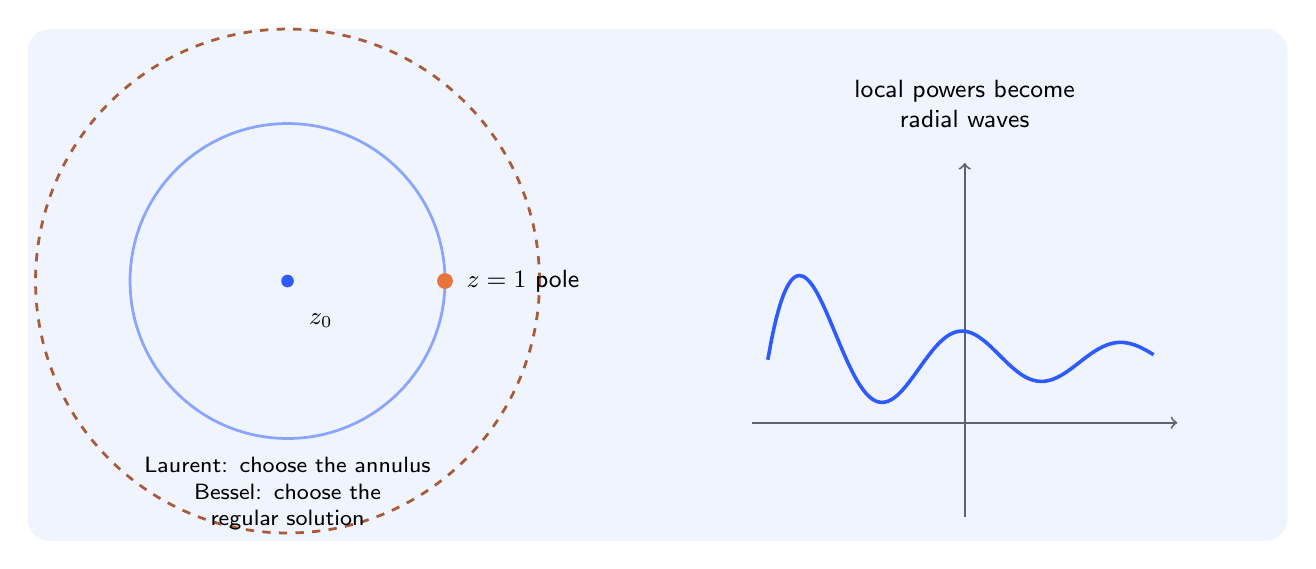
\begin{tikzpicture}[x=1cm,y=1cm]
\fill[blue!7,rounded corners=8pt] (0,0) rectangle (16,6.5);
\draw[blue!55,line width=1pt] (3.3,3.3) circle (2.0);
\draw[orange!70!ink,line width=1pt,dashed] (3.3,3.3) circle (3.2);
\fill[orange] (5.3,3.3) circle (0.10);\node[anchor=west,font=\sffamily\small] at (5.45,3.3) {$z=1$ pole};
\fill[blue] (3.3,3.3) circle (0.08);\node[anchor=west,font=\sffamily\small] at (3.45,2.8) {$z_0$};
\draw[->,ink!70,line width=.7pt] (9.2,1.5)--(14.6,1.5);\draw[->,ink!70,line width=.7pt] (11.9,.3)--(11.9,4.8);
\draw[blue,line width=1.3pt] plot[smooth,domain=9.4:14.3,samples=100] (\x,{2.3+0.9*sin(180*(\x-9.4))*(1.25/(\x-8.8))});
\node[font=\sffamily\small,align=center] at (11.9,5.55) {local powers become\\radial waves};
\node[font=\sffamily\footnotesize,align=center,text width=4cm] at (3.3,.6) {Laurent: choose the annulus\\Bessel: choose the regular solution};
\end{tikzpicture}
\vfill
\begin{keybox}
\textbf{What this guide teaches.} You will learn to (i) choose the correct Laurent annulus, (ii) derive and use the Bessel series $J_\nu$, and (iii) build multivariable Taylor polynomials from the gradient and Hessian, with error-aware worked examples.
\end{keybox}
\vspace{7mm}{\sffamily\small Prepared as a visual, typeset study note \hfill 20 September 2026}\par
\end{titlepage}

\sectiontag{01 / MAP}\section*{The three series are different tools}
A useful way to keep the ideas straight is to ask what geometry the function is responding to.
\begin{center}
\begin{tabular}{>{\raggedright\arraybackslash}p{0.27\linewidth} p{0.64\linewidth}}
\toprule
\textbf{Series} & \textbf{What it gives you}\\\midrule
Taylor in one variable & A local polynomial near one point; only nonnegative powers.\\
Laurent in one complex variable & A local expansion on an annulus; negative powers record the singular part.\\
Taylor in several variables & A polynomial in the displacement vector; the Hessian records curvature and cross-effects.\\
Bessel $J_\nu$ & A special-function series selected by a radial differential equation.\\
\bottomrule
\end{tabular}
\end{center}
\vspace{4mm}
\begin{bluebox}\textbf{Core discipline.} Before manipulating symbols, write down the centre, the singularities, and the domain where the expansion is meant to converge. A correct algebraic identity outside its domain is not a valid series solution.\end{bluebox}
\subsection*{A geometric picture}
\begin{center}
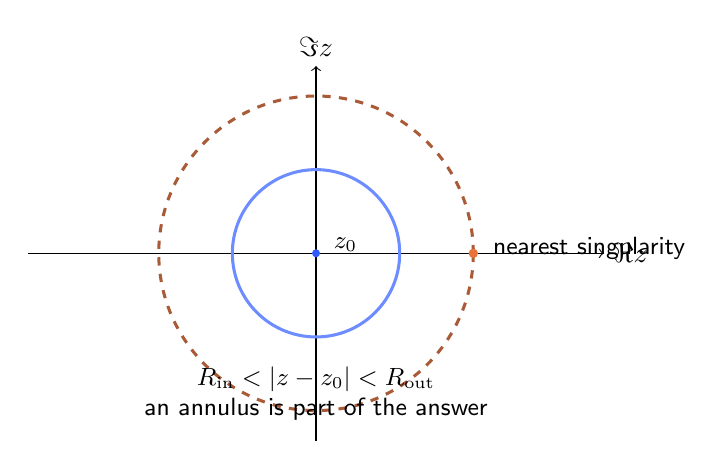
\begin{tikzpicture}[scale=.85]
\draw[->] (-4.3,0)--(4.3,0) node[right] {$\Re z$};\draw[->] (0,-2.8)--(0,2.8) node[above] {$\Im z$};
\draw[blue!70,line width=1.1pt] (0,0) circle (1.25);\draw[orange!70!ink,dashed,line width=1.1pt] (0,0) circle (2.35);
\fill[orange] (2.35,0) circle (.07);\node[font=\sffamily\small,anchor=west] at (2.5,.08) {nearest singularity};
\node[font=\sffamily\small,align=center] at (0,-2.1) {$R_{\rm in}<|z-z_0|<R_{\rm out}$\\an annulus is part of the answer};
\fill[blue] (0,0) circle (.06);\node[font=\sffamily\small,anchor=west] at (.12,.13) {$z_0$};
\end{tikzpicture}
\end{center}

\sectiontag{02 / LAURENT}\section*{Laurent series: the annulus chooses the powers}
Around $z_0$, a Laurent expansion has the form
\[
f(z)=\sum_{n=-\infty}^{\infty}a_n(z-z_0)^n,\qquad a_n=\frac{1}{2\pi i}\oint_\gamma \frac{f(\zeta)}{(\zeta-z_0)^{n+1}}\dd\zeta.
\]
The contour $\gamma$ must stay inside one annulus of analyticity. The same function can therefore have different valid expansions in different annuli.
\begin{worked}{A}
Expand $\displaystyle f(z)=\frac{1}{z(z-1)}$ about $z_0=0$.
\begin{enumerate}[leftmargin=*,itemsep=2pt]
\item For $0<|z|<1$, write $f(z)=-z^{-1}(1-z)^{-1}$.
\item Insert $\displaystyle (1-z)^{-1}=\sum_{n=0}^{\infty}z^n$.
\item Therefore $\displaystyle f(z)=-z^{-1}-1-z-z^2-\cdots$.
\end{enumerate}
The negative-power term $-z^{-1}$ is the principal part; its coefficient is the residue at $0$.
\end{worked}
\begin{orangebox}
For the outer annulus $|z|>1$, factor in $z^{-1}$ instead:
\[
\frac{1}{z(z-1)}=\frac{1}{z^2}\frac{1}{1-z^{-1}}=\sum_{n=0}^{\infty}z^{-n-2},\qquad |z|>1.
\]
\textbf{Check:} the first two terms $z^{-2}+z^{-3}$ approximate $f(2)=1/2$ by $0.375$; adding terms moves the sum toward $0.5$.
\end{orangebox}

\sectiontag{03 / BESSEL}\section*{Bessel functions: a radial ODE selects the series}
The Bessel equation is
\[
x^2y''+xy'+(x^2-\nu^2)y=0.
\]
A Frobenius trial $y=\sum_{m=0}^\infty a_m x^{m+r}$ gives the indicial equation $r^2-\nu^2=0$. The regular branch uses $r=\nu$ and the recurrence
\[
a_{m+1}=-\frac{a_m}{(m+1)(m+\nu+1)}.
\]
With $a_0=2^{-\nu}/\Gamma(\nu+1)$, this becomes
\[
J_\nu(x)=\sum_{m=0}^{\infty}\frac{(-1)^m}{m!\,\Gamma(m+\nu+1)}\left(\frac{x}{2}\right)^{2m+\nu}.
\]
For integer $\nu$, the second independent solution is $Y_\nu$, which is singular at $x=0$; $J_\nu$ is the regular choice for a finite centre.
\begin{worked}{B}
Approximate $J_0(2)$ using four terms:
\[
J_0(2)\approx 1-1+\frac{1}{4}-\frac{1}{36}=0.2222\ldots,
\qquad J_0(2)=0.2238908\ldots.
\]
The alternating terms shrink rapidly because the ratio of successive magnitudes is $\frac{x^2}{4(m+1)^2}$ when $\nu=0$.
\end{worked}
\begin{center}
\begin{tikzpicture}
\begin{axis}[width=0.86\linewidth,height=5.0cm,axis lines=left,xmin=0,xmax=18,ymin=-.65,ymax=1.05,grid=both,major grid style={line width=.2pt,draw=line},xlabel={$x$},ylabel={$J_0(x)$},tick label style={font=\scriptsize}]
\addplot[blue,line width=1.1pt] table [x index=0,y index=1] {tmp/j0.dat};
\addplot[only marks,mark=*,mark size=1.8pt,orange] coordinates {(2.4048,0)(5.5201,0)(8.6537,0)(11.7915,0)(14.9309,0)(18,0)};
\end{axis}\end{tikzpicture}
\end{center}

\sectiontag{04 / MULTIVARIABLE TAYLOR}\section*{The gradient and Hessian are the coefficient engine}
Let $f:\R^n\to\R$ and expand around $a$. With $h=x-a$,
\[
f(a+h)=f(a)+\nabla f(a)^{\!T}h+\frac12 h^T H_f(a)h+\order(\|h\|^3).
\]
For two variables, $h=(u,v)$ and
\[
\frac12h^THh=\frac12\left(f_{xx}u^2+2f_{xy}uv+f_{yy}v^2\right)_{(x,y)=a}.
\]
The mixed derivative appears twice in matrix multiplication; that factor of $2$ is a common source of errors.
\begin{keybox}
\textbf{Workflow.} (1) choose the centre $a$; (2) compute $f(a)$ and $\nabla f(a)$; (3) compute the Hessian $H_f(a)$; (4) substitute the displacement $h$; (5) state the remainder order and any convergence condition inherited from the one-variable series.
\end{keybox}

\begin{worked}{C}
Find the second-order Taylor polynomial of $\displaystyle f(x,y)=e^{x+y}$ about $(0,0)$.
\begin{align*}
f(0,0)&=1, & \nabla f(0,0)&=(1,1),\\
H_f(0,0)&=\begin{pmatrix}1&1\\1&1\end{pmatrix}.
\end{align*}
Thus
\[
T_2(x,y)=1+x+y+\frac12(x^2+2xy+y^2)=1+x+y+\frac12(x+y)^2.
\]
At $(x,y)=(0.1,0.2)$, $T_2=1.345$, while $e^{0.3}=1.3498588\ldots$; the error is about $4.86\times10^{-3}$.
\end{worked}

\sectiontag{05 / MULTIVARIABLE WORKED EXAMPLES}\section*{Two reusable expansion patterns}
\begin{worked}{D}
Expand $\displaystyle f(x,y)=\ln(1+x+2y)$ through degree 2 at $(0,0)$.
Set $u=x+2y$. Since $\ln(1+u)=u-u^2/2+\order(u^3)$,
\[
T_2(x,y)=x+2y-\frac12(x+2y)^2
=x+2y-\frac12x^2-2xy-2y^2.
\]
The series is valid when $|x+2y|<1$; geometrically, this is a strip around the origin. For $(x,y)=(0.1,-0.05)$, $u=0$ and the polynomial gives $0$, exactly matching $\ln(1)=0$.
\end{worked}
\begin{worked}{E}
Approximate $\displaystyle g(x,y)=\sqrt{1+x-y}$ at $(x,y)=(0,0)$.
Use $(1+u)^{1/2}=1+\frac12u-\frac18u^2+\order(u^3)$ with $u=x-y$:
\[
T_2(x,y)=1+\frac12(x-y)-\frac18(x-y)^2.
\]
At $(x,y)=(0.2,0.1)$, $u=0.1$ and $T_2=1.04875$; the exact value is $\sqrt{1.1}=1.0488088\ldots$. The third-order remainder is small because $|u|\ll1$.
\end{worked}
\begin{center}
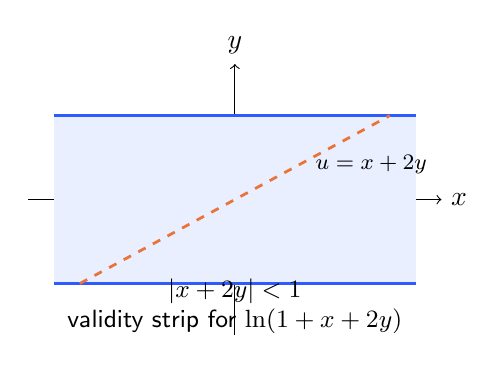
\begin{tikzpicture}[scale=.82]
\draw[->] (-3.2,0)--(3.2,0) node[right] {$x$};\draw[->] (0,-2.1)--(0,2.1) node[above] {$y$};
\fill[blue!10] (-2.8,-1.3) rectangle (2.8,1.3);
\draw[blue,line width=1pt] (-2.8,1.3)--(2.8,1.3);\draw[blue,line width=1pt] (-2.8,-1.3)--(2.8,-1.3);
\node[font=\sffamily\small,align=center] at (0,-1.65) {$|x+2y|<1$\\validity strip for $\ln(1+x+2y)$};
\draw[orange,dashed,line width=1pt] (-2.4,-1.3)--(2.4,1.3);\node[font=\sffamily\footnotesize,anchor=west] at (1.1,.55) {$u=x+2y$};
\end{tikzpicture}
\end{center}

\sectiontag{06 / SOLVE}\section*{How to use the expansions to solve functions}
\begin{enumerate}[leftmargin=*,itemsep=6pt]
\item \textbf{Match the geometry.} Use a Laurent series near an isolated complex singularity; use a multivariable Taylor polynomial near a regular point; use $J_\nu$ when the differential equation has circular/radial form.
\item \textbf{Turn the function into coefficients.} Factor rational functions into geometric-series pieces; differentiate the scalar prototype $\ln(1+u)$, $e^u$, or $(1+u)^\alpha$; or derive the Bessel recurrence from the ODE.
\item \textbf{Use the domain as a guardrail.} Record $0<|z|<1$, $|z|>1$, or $|u|<1$ next to the answer. A truncation without its domain is incomplete.
\item \textbf{Choose the truncation order from the requested accuracy.} Bound the first omitted term when the series is alternating or use a multivariable remainder estimate based on a bound for third derivatives.
\item \textbf{Validate at one point.} Compare the truncated expression with the original function numerically; this catches missing factors of $2$, wrong signs, and an expansion used outside its annulus.
\end{enumerate}
\begin{orangebox}
\textbf{Radial boundary-value recipe.} For $u_{rr}+r^{-1}u_r+\lambda^2u=0$, set $x=\lambda r$. The equation becomes Bessel's equation of order $0$, so $u(r)=A J_0(\lambda r)+B Y_0(\lambda r)$. If the centre $r=0$ is included and $u$ must stay finite, set $B=0$. If $u(R)=0$, choose $\lambda R=j_{0,k}$, a zero of $J_0$.
\end{orangebox}
\begin{center}
\begin{tabular}{p{0.25\linewidth} p{0.64\linewidth}}
\toprule\textbf{Need} & \textbf{First move}\\\midrule
Pole or isolated singularity & Find the singularity distances; choose the Laurent annulus.\\
Local approximation in $(x,y)$ & Compute $f$, gradient, Hessian at the centre.\\
Circular/radial oscillation & Test for Bessel's equation after a change of variables.\\
Accuracy estimate & Inspect the first omitted term and the domain margin.\\
\bottomrule
\end{tabular}
\end{center}

\sectiontag{07 / REFERENCE}\section*{Formula sheet and sources}
\begin{keybox}
\begin{align*}
\text{Laurent: }&f(z)=\sum_{n=-\infty}^{\infty}a_n(z-z_0)^n.\\
\text{Taylor in two variables: }&T_2=f(a)+\nabla f(a)^Th+\tfrac12h^TH_f(a)h.\\
\text{Bessel: }&x^2y''+xy'+(x^2-\nu^2)y=0.\\
\text{Regular solution: }&J_\nu(x)=\sum_{m=0}^\infty\frac{(-1)^m}{m!\Gamma(m+\nu+1)}(x/2)^{2m+\nu}.
\end{align*}
\end{keybox}
\small
\begin{enumerate}[leftmargin=*,itemsep=3pt]
\item NIST Digital Library of Mathematical Functions, §10.2, “Bessel and Hankel Functions,” \url{https://dlmf.nist.gov/10.2}.
\item NIST Digital Library of Mathematical Functions, §4.2, “Definitions and Elementary Properties” (power series and principal parts), \url{https://dlmf.nist.gov/4.2}.
\item J. W. Brown and R. V. Churchill, \emph{Complex Variables and Applications}, 9th ed., McGraw-Hill, 2014. Laurent expansions and residues.
\item J. Stewart, \emph{Calculus: Early Transcendentals}, multivariable Taylor polynomials and Hessians.
\end{enumerate}
\vfill
\begin{bluebox}\textbf{Final check.} Name the centre, show the coefficients, state the convergence region, and test one numerical point. Those four lines turn a formal expansion into a usable solution.
\end{bluebox}
\end{document}
